%%%%%%%%%%%%%%%%%%%%%%%%%%%%%%%%%%%%%%%%%%%%%%%%%%%%%%%%%%%
% EPFL report package, main thesis file
% Goal: provide formatting for theses and project reports
% Author: Mathias Payer <mathias.payer@epfl.ch>
%
% This work may be distributed and/or modified under the
% conditions of the LaTeX Project Public License, either version 1.3
% of this license or (at your option) any later version.
% The latest version of this license is in
%   http://www.latex-project.org/lppl.txt
%
%%%%%%%%%%%%%%%%%%%%%%%%%%%%%%%%%%%%%%%%%%%%%%%%%%%%%%%%%%%
\documentclass[a4paper,11pt,oneside]{report}
% Options: MScThesis, BScThesis, MScProject, BScProject
\usepackage[MScThesis,lablogo]{EPFLreport}
\usepackage{datetime}
\usepackage{amsmath}
\usepackage{amssymb}
\usepackage{xspace}
\usepackage{array}
\usepackage{lscape}
\usepackage{booktabs}
\usepackage{subcaption}
\usepackage{gensymb}
\usepackage{stmaryrd}
\usepackage{verbatim}


\usepackage{hyperref}
\usepackage{graphicx}

\title{Regional Climate Model Emulator based on Deep Learning: future SMB predictions over Antarctica}
\author{Marijn van der Meer}
\supervisor{Sophie de Roda Husman}
\adviser{Prof. Dr. sc. EPFL Martin Jäggi}
\expert{Prof. Dr. sc. TU Delft Stef Lhermitte}

\newcommand{\sysname}{FooSystem\xspace}

\begin{document}
\maketitle
\makededication
\makeacks

\begin{abstract}
The \sysname tool enables lateral decomposition of a multi-dimensional
flux compensator along the timing and space axes.

The abstract serves as an executive summary of your project.
Your abstract should cover at least the following topics, 1-2 sentences for
each: what area you are in, the problem you focus on, why existing work is
insufficient, what the high-level intuition of your work is, maybe a neat
design or implementation decision, and key results of your evaluation.
\end{abstract}

\begin{frenchabstract}
For a doctoral thesis, you have to provide a French translation of the
English abstract. For other projects this is optional.
\end{frenchabstract}

\maketoc

%%%%%%%%%%%%%%%%%%%%%%
\chapter{Introduction}
%%%%%%%%%%%%%%%%%%%%%%

\begin{itemize}
    \item Traditional U-Net is a fully convolutional CNN architecture specifically developed for biomedical image segmentation~\cite{Ronneberger2015}.  
        \item U-Net shows high performance in classification and segmentation tasks where the network is trained to predict a class for each pixel. But U-Nets are also used for image processing tasks, such as super resolution. They have been found to be particularly effective in cases where the output and inputs are of similar size. In our case, we applied it to a time series prediction task in which the network has to predict an exact value for each pixel.
    \item using attention in a CNN facilitates the network to focus on specific parts of the input. 
\end{itemize}



The introduction is a longer writeup that gently eases the reader into your
thesis~\cite{dinesh20oakland}. Use the first paragraph to discuss the setting.
In the second paragraph you can introduce the main challenge that you see.
The third paragraph lists why related work is insufficient.
The fourth and fifth paragraphs discuss your approach and why it is needed.
The sixth paragraph will introduce your thesis statement. Think how you can
distill the essence of your thesis into a single sentence.
The seventh paragraph will highlight some of your results
The eights paragraph discusses your core contribution.

This section is usually 3-5 pages.

Surface mass balance (SMB) provides mass input to the surface of the Antarctic and Greenland Ice Sheets and therefore comprises an important control on ice sheet mass balance and resulting contribution to global sea level change. As ice sheet SMB varies highly across multiple scales of space (meters to hundreds of kilometers) and time (hourly to decadal), it is notoriously challenging to observe and represent in models. In addition, SMB consists of multiple components, all of which depend on complex interactions between the atmosphere and the snow/ice surface, large-scale atmospheric circulation and ocean conditions, and ice sheet topography.~\cite{Lenaerts}

%%%%%%%%%%%%%%%%%%%%
\chapter{State of the art}
%%%%%%%%%%%%%%%%%%%%

The related work section covers closely related work. Here you can highlight
the related work, how it solved the problem, and why it solved a different
problem. Do not play down the importance of related work, all of these
systems have been published and evaluated! Say what is different and how
you overcome some of the weaknesses of related work by discussing the 
trade-offs. Stay positive!

This section is usually 3-5 pages.

\section{Regional Climate Model Emulator based on Deep Learning: Concept and First Evaluation of a Novel Hybrid Downscaling Approach \cite{Doury}}
This paper proposes a novel hybrid downscaling approach that emulates the downscaling function of a a regional climate model.

\begin{itemize}
\item RCM: EURO-CORDEX simulations based on the CNRM-ALADIN63, 1951-2100 RCP4.5 and RCP8.5
\item GCM: CNRM-CM5 used in CMIP5 → 6h frequency + sea surface temperature, sea ice cover and aerosol optical depth at monthly frequency
\item ML model learns the RCM transformation of the large-scale climate information into local-scale
\item Target variable: near surface temperature (TAS)
\item Target domain: southwest European domain
\item Historical period: 1951 to 2005
\item Scenarios (2006-2100): based on two Representative Concentration Pathways from CMIP5; RCP4.5 and RCP8.5
\end{itemize}
Computational performance:
\begin{itemize}
    \item U-Net: fully convolutional neural network algorithm
    \item Substantial computational gain regarding RCM computational cost
    \begin{itemize}
        \item 2h training on GPU + downscaling instantaneous
        \item RCM simulation involves weeks of computation on super-computer
    \end{itemize}
\end{itemize}
Training of model 
\begin{itemize}
    \item RCM can be broken down into a large scale transformation and a downscaling function
    \item Training using existing RCM simulations → learn large scale/local scale relationship in different climates and in future climate
    \item Training in perfect model framework: input and output to ML model come from same RCM simulation → focus on downscaling function
    \item Input variable: daily large-scale and low-resolution RCM information (upsampled to GCM like resolution)
    \item Output variable: daily maps of TAS at RCM resolution (~12km)
    \item Emulator is RCM-dependent as downscaling function depends on RCM choice
\end{itemize}
Results
\begin{itemize}
    \item Emulator evaluated in both perfect model (evaluation 1) and GCM worlds (evaluation 2)
    \item capture very well transformation from low resolution information to high resolution TAS
    \item robust to different sources of input
    \item succeeds very well in reproducing high resolution spatial structure and daily variability of the RCM
    \item evaluation 1 shows that emulator is able to reproduce original series almost perfectly
    \item training emulator in future climate improves its ability to reproduce warmer climate
    \item limitations in accurately simulating extreme events and complete climate change magnitude
    \item RCM-GCM large scales inconsistencies when evaluating on GCM. Does not learn to reproduce large scale transformations (because trained only on RCM)
\end{itemize}
\section{Diverging future surface mass balance between the Antarctic ice shelves and grounded ice sheet \cite{Kittel}}

\section{SmaAt-UNet: Precipitation Nowcasting using a Small Attention-UNet Architecture~\cite{smatunet}}


%%%%%%%%%%%%%%%%
\chapter{Model and methods}
%%%%%%%%%%%%%%%%

\begin{table}[!tbp]
    \centering
    \caption{}
    \renewcommand\arraystretch{1.5}
    \begin{tabular}{l>{\raggedright\arraybackslash}p{0.4\linewidth}>{\raggedright\arraybackslash}p{0.4\linewidth}}
    \toprule
        \textbf{Notation} & \textbf{Description} & \textbf{Dimensions} \\ \toprule 
        $\mathcal{D}$ & Input Domain & $\llbracket 1, I \rrbracket \times \llbracket 1, J \rrbracket$   \\
        $\mathcal{E}$ & Target Domain & $\llbracket 1, K \rrbracket \times \llbracket 1, L \rrbracket$   \\
        $(i,j)$ & Spatial indexes over
        input grid & $\mathcal{D}$   \\
        $(k,l)$ & Spatial indexes over
        target grid & $\mathcal{E}$   \\
        $X$ & Input: set of 2D variables over $\mathcal{D}$ & $T \times \llbracket 1, I \rrbracket \times \llbracket 1, J \rrbracket \times C_1$   \\
        $Z$ & Input: set of 1D variables over $\mathcal{D}$ & $T \times C_2$   \\
        $Y$ & Target: surface mass balance over $\mathcal{E}$ & $T \times \llbracket 1, K \rrbracket \times \llbracket 1, L \rrbracket$  \\
        $t$ & Monthly temporal index & $T$   \\
        $x$ & 2D variables index & $C_1$   \\
        $z$ & 1D variables index & $C_2$ 
        \\
        $F$ & Downscaling function of the RCM & 
        \\
        $\hat{F}$ & Emulator: Estimation of F & 
        \\
        $\operatorname{UPRCM}$ & GCM-like: upscaled RCM to GCM resolution & 
        \\
\bottomrule
    \end{tabular}
        \subcaption*{\small Table~\ref{tab:notations}. Notations used in this paper.}
            \label{tab:notations}
\end{table}

\begin{itemize}
\item \textbf{Global idea}: the RCM-emulator $\hat{F}$ uses a neural network architecture to estimate the downscaling function $F$ in 
\begin{equation}\label{eq:emulator-equation}
    Y = \operatorname{F}(X) \;\;\;\; X\subset\mathcal{D}, Y\subset\mathcal{E}
    \end{equation}
where $X$ are low-resolution variables from a global climate simulation over an input domain $\mathcal{D}$ and $Y$ is a high resolution surface variable inside a regional climate simulation over a target domain $\mathcal{E}$. 
\item Flow of model and methods section: 
\begin{itemize}
    \item Data: climate models used -> target and input domains -> variables chosen (input features)
    \item Model: architecture -> perfect model framework (creation of UPRCM) -> training flow (on GCM and UPRCM) -> evaluation flow
\end{itemize}
\end{itemize}

\section{Data}\label{sec:data}
\subsection{Climate model}
\begin{itemize}
    \item RCM: RCM variable emulated by $\hat{F}$ is the monthly surface mass balance (SMB) values from MAR(ACCESS1.3), a regional downscaling of the global climate model ACCESS 1.3 (CMIP5~\cite{ACCESS13, CMIP5}) by the Modèle Atmosphérique Régional (MAR). 
    \item MAR: MAR is known for its accurate modelling of physical processes in the polar regions such as surface mass balance, air-snow interactions, and atmospheric circulation over ice sheets~\cite{MAR}. 
    \item Why: We chose MAR(ACCESS 1.3) because according to the studies conducted in~\cite{Kittel, Agosta2015} that compared several climate models, ACCESS1.3 and more specifically MAR(ERA5) were the global and regional climate models that most accurately represented the present Antarctic climate in comparison to ERA-Interim and MAR(ERA5). 
    \item Time-frame: historical values from 1980-2006 and future climate simulation RCP 8.5~\cite{Moss2010} from 2006-2100. 
    \item Grid and resolution: RCM grid in south polar stereographic coordinates of $35 \times 35$ km resolution. GCM resolution of 1.25° latitude by 1.875° longitude (approximately $68 \times 206$ km), using a staggered Arakawa C grid~\cite{ACCESS13, ACCESS13_2}. 
    \item Reprojection: to have both climate models in the same projection system, we re-project the GCM to polar stereographic coordinates (see Annex for details [REF ANNEX]). 
\end{itemize}

\begin{figure}[!t]
  \centering
  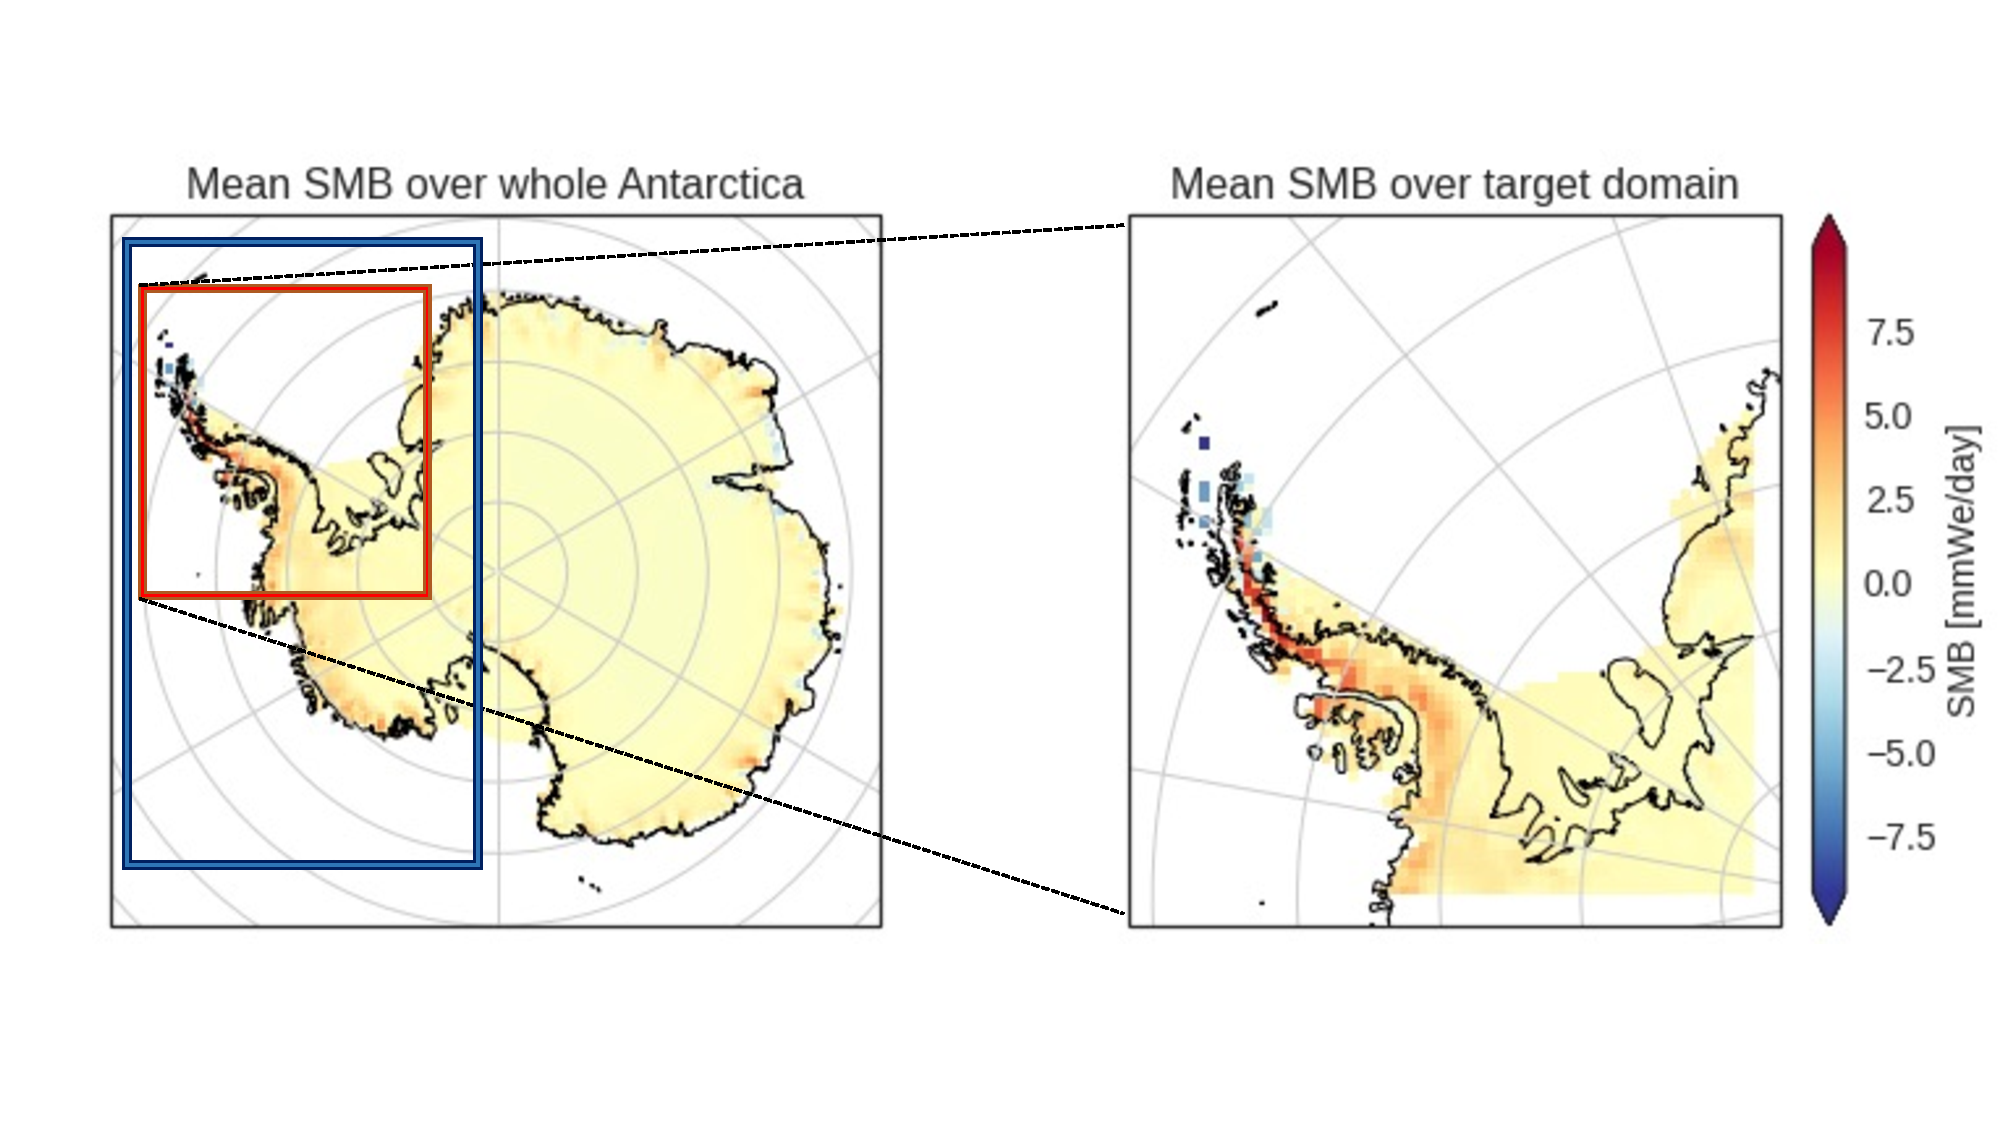
\includegraphics[width=\columnwidth]{images/domains.pdf}
  \caption []{\small Mean surface mass balance over Antarctica (left) and Antarctic Peninsula (right) from 1990-2100. Regions chosen as target domain $\mathcal{E}$ (in red) and input domain $\mathcal{D}$ (in blue) for Emulator.}
  \vspace{-3mm}
    \label{fig:region-of-choice}
\end{figure}


\subsection{Target and input domain}
\begin{itemize}
    \item Target domain: The target domain used for this model is a grid box of $64 \times 64$ at 35km resolution that contains the Antarctic Peninsula in West Antarctica. 
    \item Antarctic peninsula: 
    \begin{itemize}
        \item The Antarctic Peninsula is the most northerly part of Antarctica
        \item It covers approximately 5 million square kilometres and is mainly covered by ice. Major ice shelves include the Larsen and Ronne ice shelves.
        \item It is very mountainous, with its highest peaks rising to about 3'000 m
        \item temperature: it has the mildest climates within this continent. Its temperatures are warmest in January, averaging 1 to 2$\degree C$, and coldest in June, averages from -15 to -20$\degree C$~\cite{AntarcticPeninsula}
        \item precipitation: varies greatly within the Antarctic Peninsula. The tip of peninsula has highest levels of precipitation with 35–50cm per year. On the west coast and along its northeast coast, occasional rain leaves precipitation at 35cm. Along the east coast and the interior of Antarctica, climate is drier with precipitation that ranges from 10-15 cm~\cite{antarctic-climate, antarctic-climate-2}
    \end{itemize} 
    \item Why this region: 
    \begin{itemize}
        \item Because of the specific patterns of climate variables such as temperature and precipitation, the Antarctic Peninsula has a high annual and geographical variability in SMB values. 
        \item This shows when looking at mean SMB values as in Fig.~\ref{fig:region-of-choice}. The tip of the peninsula and its west coast show higher values than the rest. Mean SMB values range from -9.2 to 9.9 mmWe/day and the extremes observed in this region over the whole time-frame of 1980-2100 are a minimum of -59.0 mmWe/day and a maximum of 30.2 mmWe/day. 
        \item All of this makes this region very interesting to us because we want to see how the Emulator adapts to different annual patterns of SMB over our target domain.  
    \end{itemize}
    \item Input domain: $48\times25$ grid box (Fig.~\ref{fig:region-of-choice}) defined around the target domain that is resized to $32\times 32$ by bilinear interpolation so as to give the model a square input.
\end{itemize}


\subsection{Features}\label{subsec:features}
\begin{itemize}
    \item The Emulator receives as input features $(X, Z)$ that consist of two-dimensional variable $X$, and one-dimensional $Z$ (Table~\ref{tab:features}). 
    \item X: The two-dimensional feature $X$ contains eight different atmospheric variables measured daily at (near) surface level. After a monthly mean aggregation, the frequency of variables is monthly.
    \item Normalisation of X: These variables are normalised according to their spatial mean $\bar{X}_{t,x}$ and standard deviation $\sigma(X_{t,x})$:
    \begin{equation}\label{eq:normalisation-X}
    \tilde{X}_{t,i,j,x} = \frac{X_{t,i,j,x}-\bar{X}_{t,x}}{\sigma(X_{t,x})} \;\;\;\; t\in T, \forall (i,j) \in \mathcal{D}, x\in C_1
\end{equation}
    \item (These eight variables were present both in our RCM and GCM data. In terms of feature selection, we decided to follow the same procedure as in~\cite{Doury} and give all available variables to the model and let it find the right combination to be used [COMPLETE WITH FEATURE SELECTION RESULTS].)
    
\item Z: The one-dimensional variable $Z$ includes time-series of spatial means $\bar{X}_{t,x}$ and standard deviations $\sigma(X_{t,x})$ for each atmospheric variable $x\in C_1$.
\item Temporal encoding of Z: 
\begin{itemize}
    \item because the 2D variables $X$ are normalised at each time step by their spatial mean and so don’t carry any temporal information.
    \item It also includes a cosinus, sinus vector to encode the information about the month of the year.
    \begin{equation}
        \operatorname{cos}\left(\frac{2\pi t}{12}\right);\; \operatorname{sin}\left(\frac{2\pi t}{12}\right) \;\;\;\; \forall t\in T
    \end{equation}
\end{itemize}

\item Overall Z: 
\begin{equation}
    Z = \left[ \bar{X}_{t\in T, x\in C_1}, \sigma\left(X_{t\in T, x\in C_1}\right), \operatorname{cos}, \operatorname{sin} \right] \subset T \times C_2
\end{equation}

\item Normalisation of Z: each of the spatial means $\bar{X}_{t,x}$ and standard deviations $\sigma(X_{t,x})$ in Z are normalised according to a reference period ($\mathrm{ref}=$1980-2000)~\cite{Doury}:
\begin{equation}\label{eq:normalisation-Z}
    \tilde{Z}_{t,z} = \frac{Z_{t,z}-\bar{Z}_{\mathrm{\mathrm{ref}},z}}{\sigma(Z_{\mathrm{ref},z})} \;\;\;\; t\in T, z\in C_2
\end{equation}
where $\bar{Z}_{\mathrm{ref},z}$ and $\sigma(Z_{\mathrm{ref},z})$ are respectively the temporal mean and standard deviation of the spatial means or standard deviations of $X_{\mathrm{ref}, x} \subset T_{\mathrm{ref}}\times C_1$.
\end{itemize}

\begin{table}[tbp]
    \centering
    \caption{}
    \renewcommand\arraystretch{1.5}
    \begin{tabular}{l>{\centering}p{0.1\linewidth}>{\centering}p{0.2\linewidth}>{\centering\arraybackslash}p{0.2\linewidth}}
    \toprule
        \textbf{Variable Name} & \textbf{Variable Notation} & \textbf{Units} & \textbf{Dimensions} \\ \toprule
        \textbf{2D variables} & & & \\ \bottomrule 
        Northward Wind & NW & $[ms^-1]$ & $ \mathcal{D}$   \\ 
        Eastward Wind & EW & $[ms^-1]$ & $ \mathcal{D}$ \\
        Downwelling Shortwave Radiation & SWD & $[Wm^{-2}]$ & $ \mathcal{D}$ \\
        Downwelling Longwave Radiation & LWD & $[Wm^{-2}]$ & $ \mathcal{D}$ \\
        Specific Humidity & QQP & $[g/Kg]$ & $ \mathcal{D}$ \\
        Temperature & TT & $[\degree]$ & $ \mathcal{D}$ \\
        Precipitation & PR & $[mmWe/day]$ & $ \mathcal{D}$  \\
        Pressure & PR & $[hPa]$ & $ \mathcal{D}$  \\
        \toprule
         \textbf{1D variables} & & & \\ \bottomrule
        Spatial mean of 2D variables & $\bar{X}_{x}$ & & $[C_1]$ \\ 
        Spatial std of 2D variables & $\sigma\left(X_{x}\right)$ & & $[C_2]$ \\
        Seasonal Indicators & & & $[2]$\\ \bottomrule
        
    \end{tabular}
        \subcaption*{\small Table~\ref{tab:features}. Two and one-dimensional input features given to the model. Each feature is measured (near) surface and a monthly mean aggregation.}
            \label{tab:features}
\end{table}


\section{Model}\label{sec:model}

\begin{figure}[!t]
  \centering
  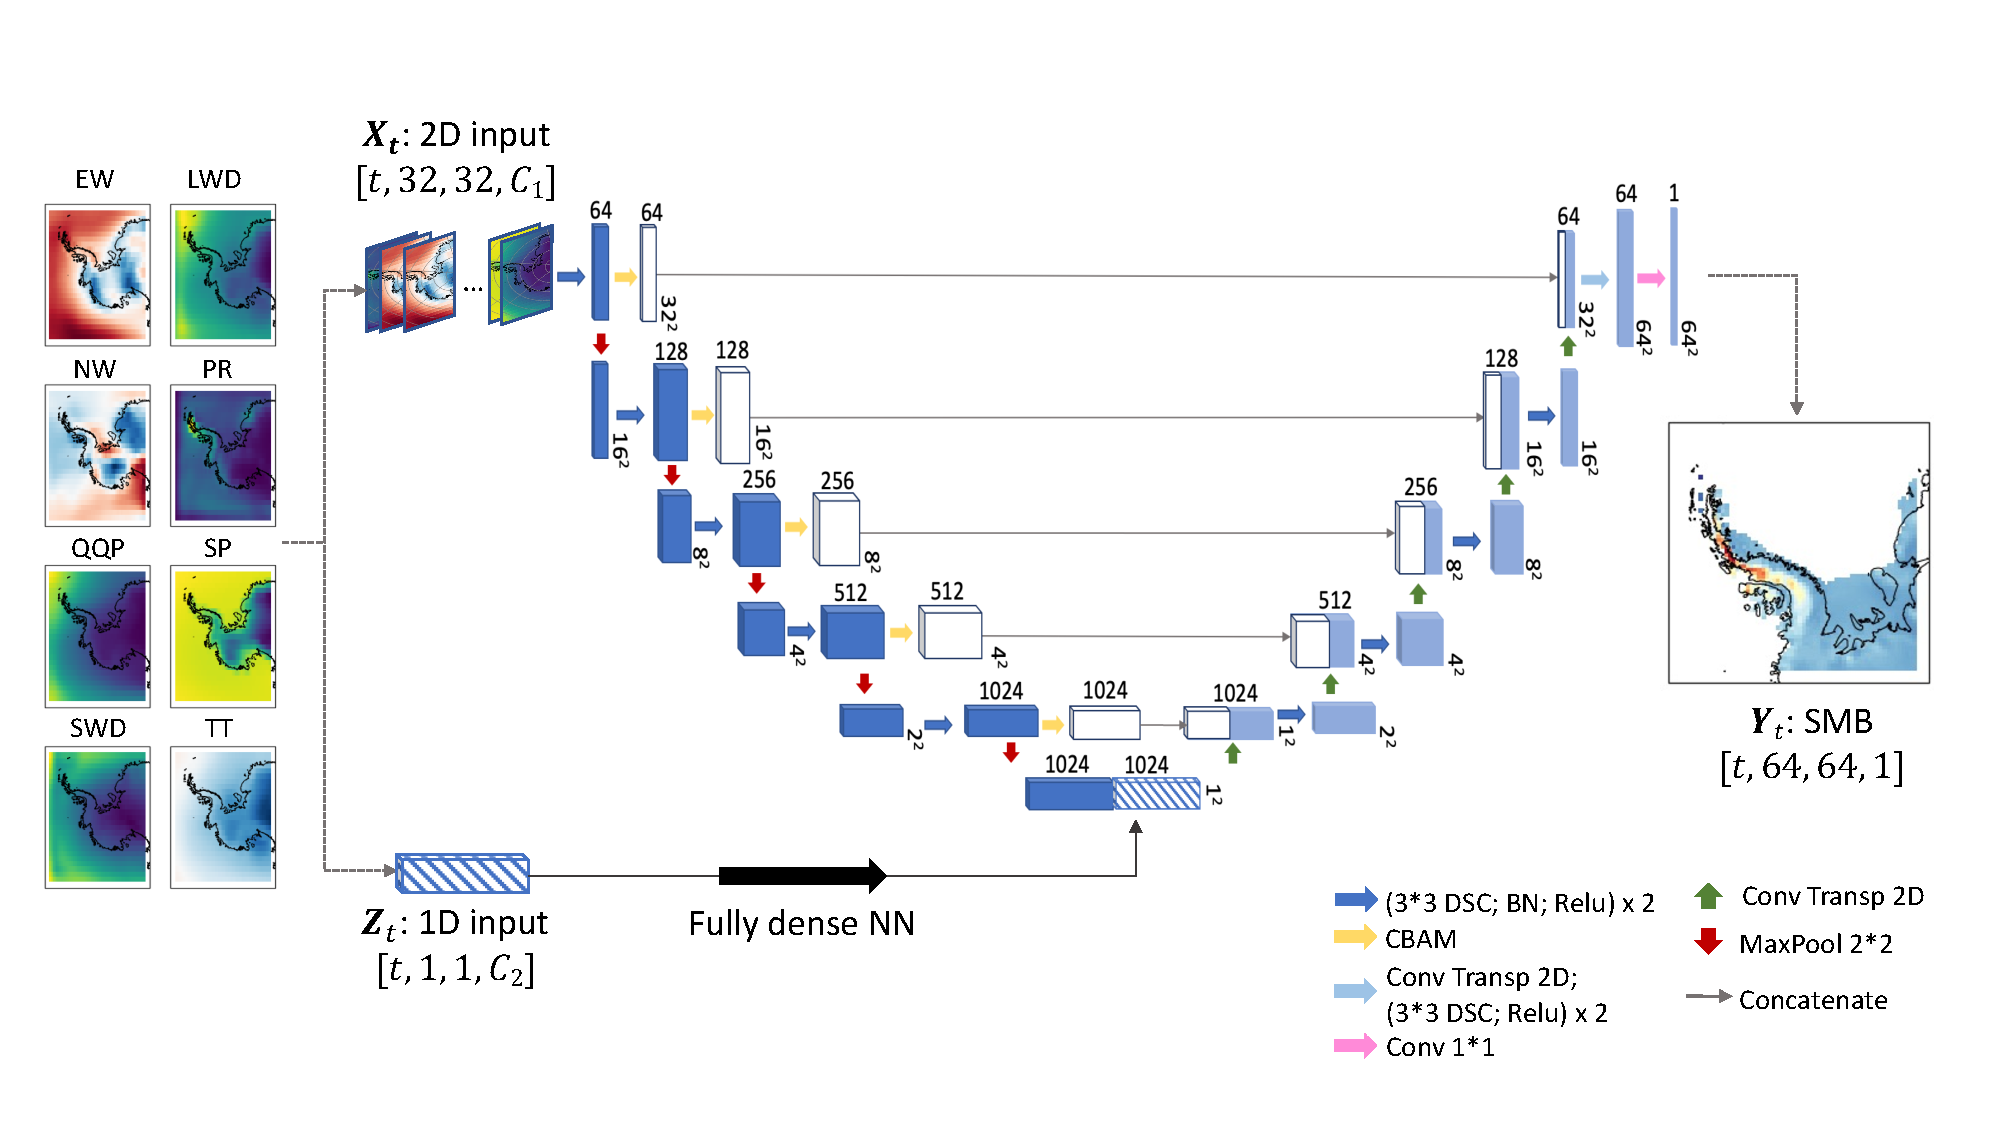
\includegraphics[width=\columnwidth]{doc/Thesis-latex/images/unet-with-data.pdf}
  \caption []{\small Illustration of an observation at time-step $t$. Left: 2D input variables $X_t$ on the input domain with its corresponding 1D variable $Z_t$. Right: target surface mass balance (SMB) $Y_t$ on the target domain. Middle: scheme of the U-Net architecture used for this paper. }
  \vspace{-3mm}
  \label{fig:example-features}
\end{figure}

\subsection{Architecture}\label{subsec:architecture}
\begin{itemize}
    \item The Emulator's architecture extends the U-Net used to emulate near-surface temperature in~\cite{Doury} with mechanisms from the SmaAt-UNet model~\cite{smatunet} (Fig.~\ref{fig:example-features}).
     \item SmaAt-UNet: SmaAt-UNet extends the traditional U-Net architecture~\cite{unet} with CBAM attention mechanism and depthwise-separable convolutions instead of regular convolutional operations. 
    \item Architecture: 
    \begin{itemize}
    \item The network is U-shaped as it is divided into a down-sampling/encoder section that forms the left side and an up-sampling/decoder on the right.
    \item Encoder: the Encoder consists of double convolution (blue arrows) followed by max-pooling (red arrows). This process halves the image size and doubles the number of channels. Instead of the traditional U-Net convolutional operations, the Emulator uses depthwise-separable convolutions (DSC), designed to reduce the number of parameters~\cite{smatunet}.
    \item Bottom of U-Net: At the bottom of the U-Net, encoded spatial information from $X_t$ and temporal information from $Z_t$ are concatenated. The corresponding 1D input $Z_t$ of $X_t$ first goes through a fully dense neural network to reach the same number of channels as the output of the last layer of the Encoder. Then, it is concatenated with the Encoder output at the bottom of the “U”. This constrains the U-Net to give equal importance to the spatial and temporal inputs before starting the decoding path and generating the high-resolution SMB image~\cite{Doury}. 
    \item Decoder: three parts; a 2D transposed convolution operation (green arrows) to double the image size, a concatenation of the resulting feature maps with the previous Encoder’s attention maps (white blocks) via skip-connections (grey arrows), and lastly a double depthwise-separable to half the number of channels (blue arrows). 
    \item Skip-connections: skip-connections between layers (grey arrows) make it possible to skip large sections if required and create a smoother loss surface. 
    \item  Last layers: up-sampling layer (light blue arrow) in order to reach target size ($64\times 64$) and $1\times1$ convolution (pink arrow) to change the number of channels from $64$ to $1$, and outputs a single image representing the SMB values predicted by the network at time-step $t$.
    \item Attention: Convolutional block attention modules (CBAMs, yellow arrow)~\cite{smatunet} are placed after each double convolution in the Encoder and used to detect important features over the channels and spatial regions of the inputs. In CBAMs, the attention mechanism is first applied over the channels of the image and then the spatial dimension. Note that the input to the next layer of the Encoder is not the attention feature map (white block) but the convoluted and downsampled image of the previous layer (dark blue block). This way, the original image features are preserved throughout the Encoder layers. Finally, the attention blocks are fed through skip-connections to the corresponding Decoder layer to be concatenated~\cite{smatunet}. Contrary to the DSC convolutions used in the Encoder and Decoder, CBAMs use regular convolutions.  
    \end{itemize}
    \item Code: Architecture implemented in PyTorch 1.11 and available on LINK GITHUB
\end{itemize}

\subsection{Perfect model framework}\label{subsec:perfect-model}
\begin{itemize}
    \item The authors of~\cite{Kittel} trained their Emulator in a \textit{perfect model framework} where both inputs and outputs of the Machine Learning model come from the same RCM simulation. 
    \item Why:
    \begin{itemize}
        \item Their Emulator aims to learn the downscaling function $F$ of the RCM in Eq.~\ref{eq:emulator-equation}.
        \item For this, the model needs perfect consistency (high temporal and spatial correlation) between the low-resolution inputs $X$ and the high-resolution target $Y$. Otherwise, the emulator will try to learn a non-existing or non-exact relationship between $X$ and $Y$.
        \item Because of large-scale biases and inconsistencies between GCM and RCM variables, a perfect consistency cannot be guaranteed.
    \end{itemize}
    \item Creation of UPRCM: 
    \begin{itemize}
        \item To test the effect of this training framework on our Emulator, we follow the procedure outlined in~\cite{Doury} and create "GCM-like" features ($\operatorname{UPRCM}$).
        \item In a first step, RCM features are upscaled to GCM resolution ($68\times206$ km) through conservative interpolation. 
        \item In a second step, the upscaled RCM features are smoothed with a $3\times3$ moving average filter. This filter conserves the GCM grid, but each point now contains smoother information, and this further ensures the removal of local-scale information that might persist through the upscaling~\cite{Doury, Klaver2020}.
    \end{itemize}
\end{itemize}

\section{Training}\label{subsec:training}
\begin{itemize}
    \item Input to model: As aforementioned in~\ref{subsec:features}, each observation given to the Emulator are features $X_t$ and $Z_t$ for a month $t$. $X_t \in I \times J \times C_1$ is an array, where the two first dimensions are the spatial coordinates of the input domain, and the number of channels $C_1$ are the different atmospheric variables chosen as predictors. $Z_t \in C_2$ is its corresponding temporal encoding (Fig.~\ref{fig:example-features}).
    \item UPRCM and GCM: we train two Emulators. The first Emulator ($\operatorname{\hat{F}_U}$) follows the perfect model framework (~\ref{subsec:perfect-model}) and is trained using low-resolution inputs coming from the RCM simulation (UPRCM). In a second step, we train another Emulator ($\operatorname{\hat{F}_G}$) with coarse features that directly come from the GCM. 
    \item Why: The perfect model framework allows us to evaluate how the U-Net performs when it has to learn only the downscaling function of the RCM. In the second training set, we want to see whether the model can learn the underlying dynamics, despite inconsistencies and biases, between GCM and RCM. 
    \item Loss: 
    \begin{itemize}
        \item In~\cite{Doury}, the authors propose to view the problem as a regression and used Mean Squared Error (MSE) as a loss function. For our Emulator, using MSE performed poorly and it did not seem appropriate to our setting. 
        \item As aforementioned, the scales of SMB values vary greatly across the target domain. For example, dry inland points have very small annual variations of SMB with maximum values reaching under 2 [mmWe/day], while a point on the west coast may reach low extremes of -20 [mmWe/day]. In this unbalanced setting, MSE will penalize the ill-fitting of low SMB regions less than for points with high annual SMB.  
        \item For this reason, we need the points to be brought on the same scale and so we chose to use a normalised RMSE (NRMSE) loss. Normalizing the RMSE facilitates the comparison between datasets with different scales such as is our case. At each pixel location $p$ in the target domain $\mathcal{E}$, we calculate the NRMSE between the predicted values $\widehat{Y_{p}}$ and the ground truth $Y_{p}$:
        \begin{align}
        \operatorname{NRMSE}\left(Y_{p},\widehat{Y_{p}}\right) &= \frac{RMSE}{Y_{\max} - Y_{\min}} \\
         &=\frac{\sqrt{\frac{1}{T}\sum_{t}(\hat{y}_{p}^{t}-y^{t}_{p})^2}}{Y_{\max} - Y_{\min}}   \;\;\;\; \forall p \in \mathcal{E} 
        \end{align}
        where $\hat{y}_{p}^{t}$ is the SMB value predicted at location $p\in \mathcal{D} $ and time step $t\in T$ and $Y_{\max}$, $Y_{\min}$ are respectively the maximum and minimum value of SMB over $T$ and $\mathcal{E}$.
        \item Other parameters: The model is trained with features from 1980-2090, a batch-size of 32 and over 50 epochs using early stopping and a learning-rate scheduler that reduces the learning rate on loss plateaus (starting with $\operatorname{LR} = 0.005$). With this setting, the Emulators $\hat{F}_U$ and $\hat{F}_G$ respectively train for 34 and 36 epochs before stopping. 
    \end{itemize}
\end{itemize}

\section{Evaluation}\label{sec:evaluation}
% evaluation framework
\begin{figure}[!t]
  \centering
  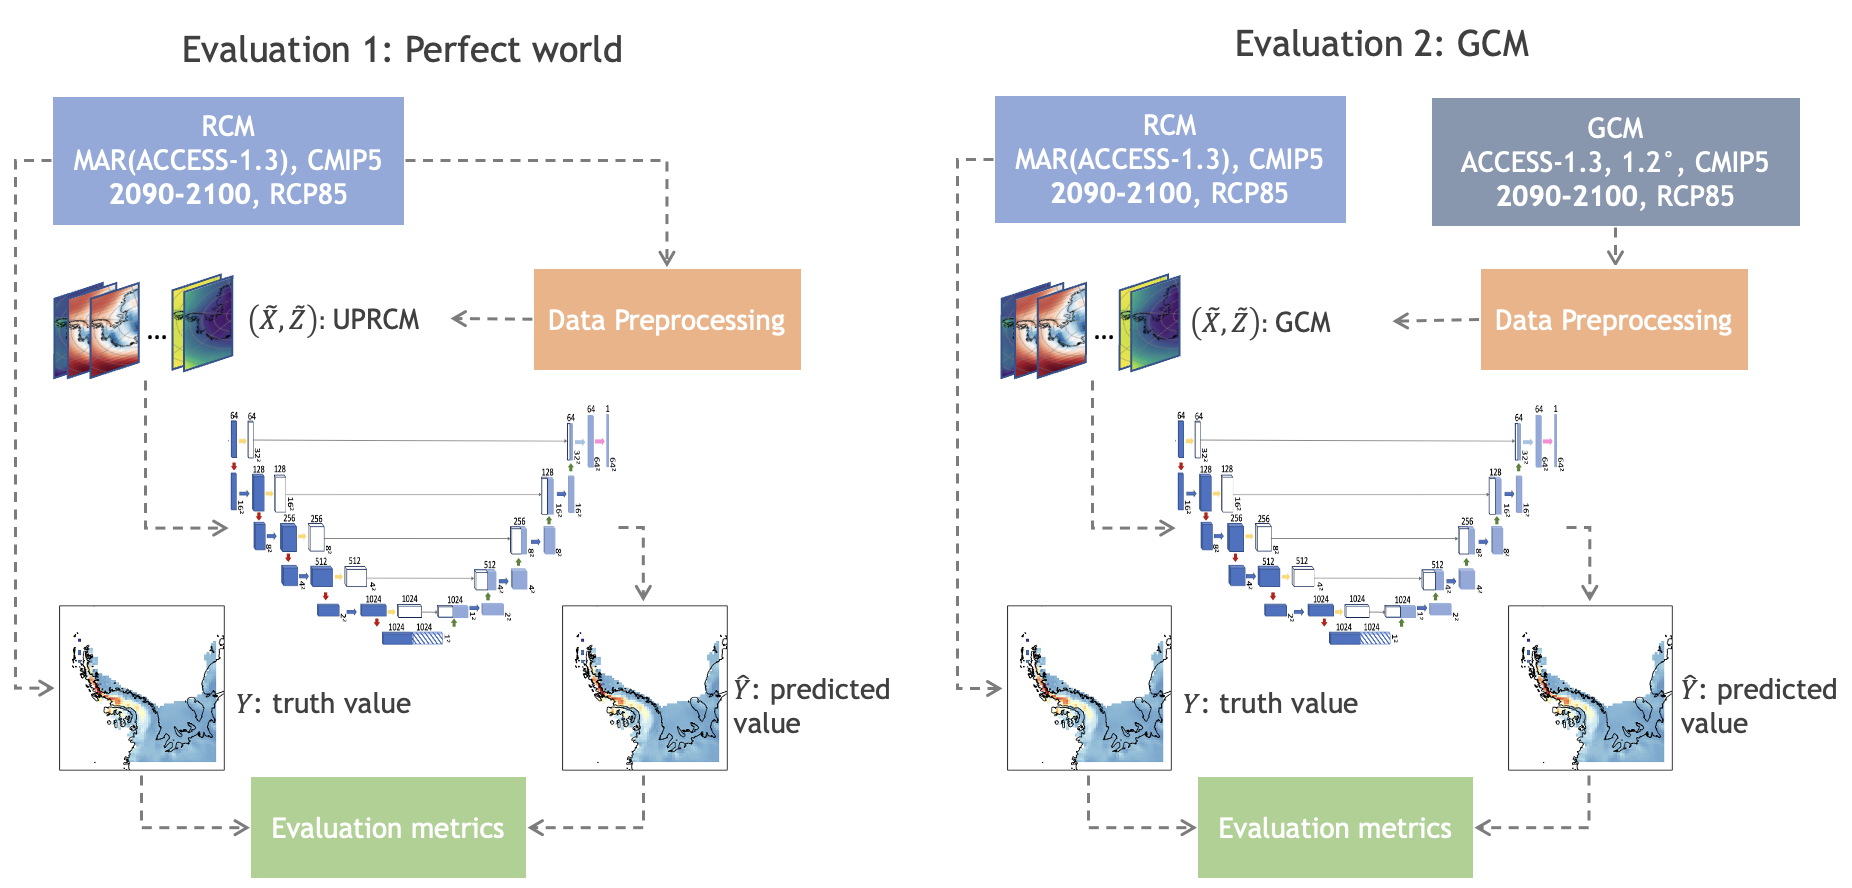
\includegraphics[width=\columnwidth]{images/evaluation_framework.png}
  \caption []{\small Evaluation framework. Left: perfect world scenario where both the input (UPRCM) and output of the model come from the RCM simulation. Right: GCM scenario where input comes from GCM and output from RCM. Evaluation metrics used described in~\ref{subsec:evaluation-metrics}.}
  \vspace{-3mm}
  \label{fig:evaluation-framework}
\end{figure}

\subsection{Framework}\label{subsec:evaluation-framework}
As previously mentioned in~\ref{subsec:perfect-model-training}, the model is trained in a perfect model framework, where both its low resolution inputs and high resolution output come from the same regional climate model.
\begin{itemize}
\item If RCP 4.5 not available, train model on 90\% of time series i.e. from 1980 till 2080 and evaluate on future scenario 2080-2100. 
    \item If RCP 4.5. avaible, train on RCP 8.5 and evaluate on whole time series of RCP 4.5.
    \item In a second evaluation step, evaluate with inputs from GCM 
\end{itemize}


\subsection{Evaluation metrics}\label{subsec:evaluation-metrics}
At each position $p$ in domain $\mathcal{D} $ of the regional climate model grid, the truth series ($Y_{p}$) from the regional climate model are compared the predicted values $\widehat{Y_{p}}= \theta(Y_{p})$ by the emulator $\theta$. For this, we use the same statistical scores the authors of~\cite{Doury} used to evaluate their downscaling model. Each of these metrics is computed over the complete period from $t_{0}=31.01.1980$ to $t_{N}=31.12.2100$:
\subsubsection{RMSE}\label{subsubsec:rmse}
The Root Mean Squared Error (RMSE) is a measure of the difference between predictions of an estimator and the observed values. RMSE is the square root of the average of squared differences between prediction and actual observation. It is also defined as the square of the Mean Squared Error (MSE):
\begin{align}
        \operatorname{RMSE}\left(Y_{p},\widehat{Y_{p}}\right) & = \sqrt{\operatorname{MSE}\left(Y_{p},\widehat{Y_{p}}\right)} \\ & = \sqrt{\frac{1}{T}\sum_{t}(\hat{y}_{p}^{t}-y^{t}_{p})^2} & \forall p \in \mathcal{D} 
\end{align}
where $\hat{y}_{p}^{t}$ is predicted SMB value and $y^{t}_{p}$ the true SMB value at location $p\in \mathcal{D} $ and time step $t$. The amplitudes of SMB time series varies according to geographical location i.e., some locations that are very dry may have SMB values that vary between 0 and 1 mmWe/day while others may go up to 10 mmWe/day. For this reason, we also compute the normalised RMSE (NRMSE):
\begin{align}
        \operatorname{NRMSE}\left(Y_{p},\widehat{Y_{p}}\right) & = \frac{\operatorname{RMSE}\left(Y_{p},\widehat{Y_{p}}\right)}{Y_{max}(p) - Y_{min}(p)} \\ & = \frac{\frac{1}{T}\sum_{t}(\hat{y}_{p}^{t}-y^{t}_{p})^2}{Y_{max} - Y_{min}} & \forall p \in \mathcal{D} 
\end{align}
where $Y_{max}$ and $Y_{min}$ are respectively the maximum and minimum true SMB values over the whole domain $\mathcal{D}$. 


\subsubsection{Pearson correlation}\label{subsubsec:pearson}
Pearson correlation coefficient measures how two continuous signals co-vary over time and indicate the linear relationship as a number between -1 (negatively correlated) to 0 (not correlated) to 1 (perfectly correlated).
\begin{align}
    \rho\left(Y_{p},\widehat{Y_{p}}\right) = \frac{\operatorname{cov}(Y_{p},\widehat{Y_{p}})}{\sigma_{Y_{p}}\sigma_{\widehat{Y_{p}}}} \;\;\;\; \forall p \in (x,y)
\end{align}
where $\operatorname {cov}$  is the covariance and  $\sigma$ is the standard deviation.

\subsubsection{Wasserstein distance}\label{subsubsec:wasserstein}
The Wasserstein distance is the numerical cost of an optimal transportation problem i.e., the cost of
the optimal transport plan~\cite{villani} for moving the mass in the predicted
measure to match that in the target~\cite{wasserstein1}. It measures the distance between two probability density functions $f(\cdotp)$, in our case $f(Y_p)$ and $f(\widehat{Y_p})$.
\begin{equation}
    \operatorname{W}\left(f(Y_p),f(\widehat{Y_p})\right) = \sum_{t}|y^{t}_{p}-\hat{y}_{p}^{t}| \;\;\;\; \forall p \in (x,y)
\end{equation}
 where $\hat{y}_{p}^{t}$ is the SMB value predicted at location $p\in (x,y)$ and time step $t$.

\subsubsection{Variance ratio}\label{subsubsec:variance-ratio}
 The variance ratio measures the performance of the emulator in reproducing local monthly variability. 
 \begin{equation}
     \operatorname{V}(Y_{p},\widehat{Y_{p}}) = \frac{\operatorname{Var}(\widehat{Y_{p}})}{\operatorname{Var}(Y_{p})}\cdot100
 \end{equation}
 where $\operatorname{Var}(Y)$ is the variance $\sigma^2$ of sample $Y$. The authors of~\cite{Doury} express this measure as a percentage. 



%%%%%%%%%%%%%%%%%%%%
\chapter{Results}
%%%%%%%%%%%%%%%%%%%%

\section{Comparison between $\hat{F}$ on UPRCM and GCM}

\subsection{Evaluation metrics}

\begin{itemize}
    \item Close in Pearson correlation but higher difference in Wasserstein and RMSE where F(UPRCM) is closer to truth. Indicates Emulator on GCM gets idea of time series but misses amplitude.
    \item Ref Fig.~\ref{fig:evaluation-GCM-RCM}
\end{itemize}

% evaluation metrics
\begin{figure}[thb]
  \centering
  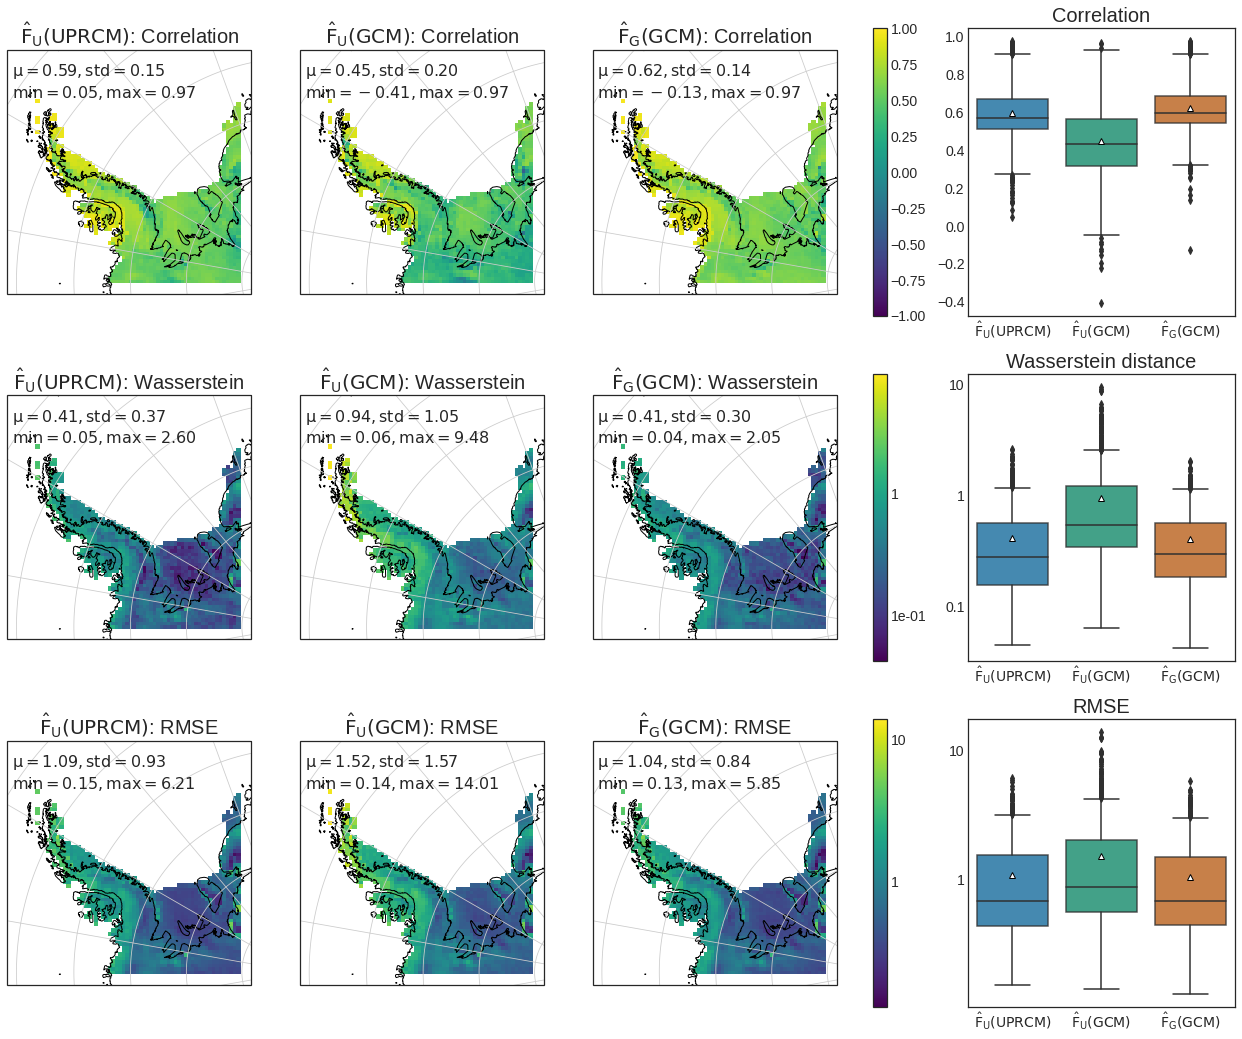
\includegraphics[width=\columnwidth]{doc/Thesis-latex/images/results/metrics_RCM_GCM.png}
  \caption []{\small Evaluation of Emulator trained on UPRCM ($\hat{F}$) or on GCM ($\hat{G}$) and using respectively UPRCM ($\operatorname{\hat{F}(UPRCM)}$) and GCM as low-resolution input ($\operatorname{\hat{F}(GCM)}$, $\operatorname{\hat{G}(GCM)}$). Test period (2090-2100). At each position $p$ in target domain $\mathcal{E}$, the truth series over the test period are compared to predicted SMB values $\operatorname{\hat{F}(\cdot)}$ and $\operatorname{\hat{G}(\cdot)}$. Right: box plot of evaluation metric values, extending from lower to upper quartile, with a line at the median and triangle at the mean. From top to bottom: Pearson correlation, Wasserstein distance and RMSE (\ref{subsubsec:rmse}). Legend: spatial mean ($\operatorname{\mu}$) and standard deviation ($\operatorname{std}$) of metric over $\mathcal{E}$. }
  \vspace{-3mm}
  \label{fig:evaluation-GCM-RCM}
\end{figure}


\subsection{Geoplots}

% SMB predictions over geoplots
\begin{figure}[thb]
  \centering
  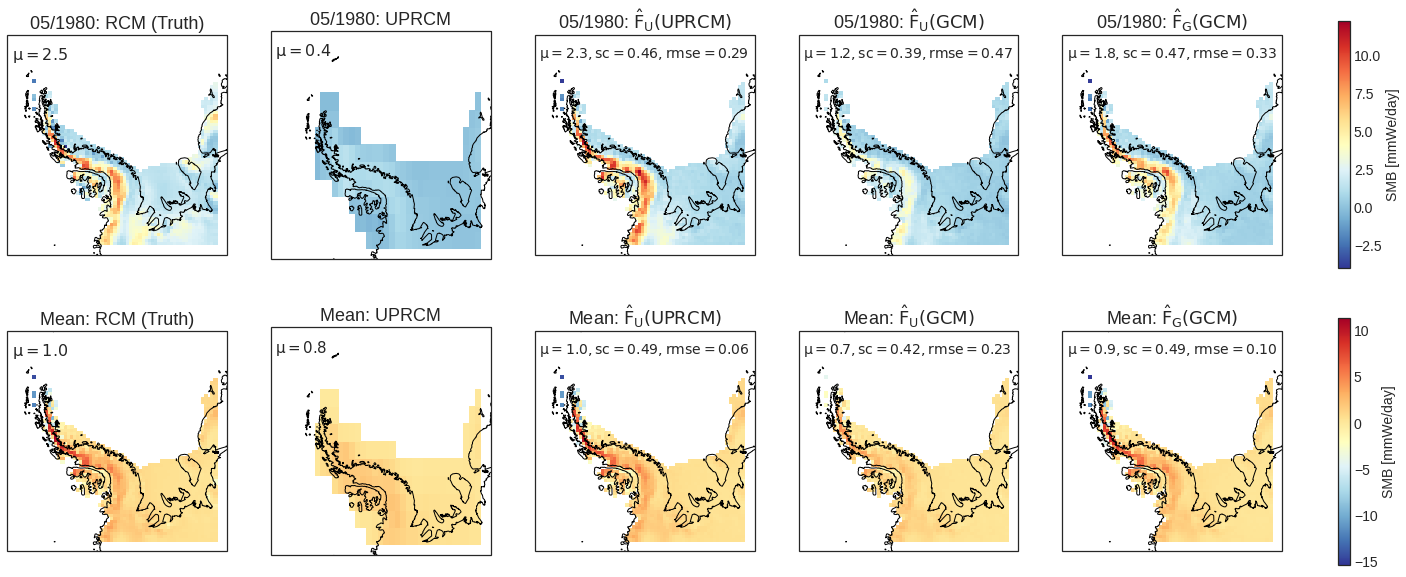
\includegraphics[width=\columnwidth]{doc/Thesis-latex/images/results/geoplots_RCM_GCM.png}
  \caption []{\small SMB on a random month (05/1980) (top) and averaged over the test period (bottom) over $\mathcal{E}$. From left to right: SMB as in the UPRCM, true RCM, $\operatorname{\hat{F}(UPRCM)}$ and $\operatorname{\hat{F}(GCM)}$. Legend: spatial mean ($\mu$) over $\mathcal{E}$ and spatial correlation ($\operatorname{sc}$) and spatial RMSE ($\operatorname{rmse}$) between the emulated and true SMB pixel values.}
  \vspace{-3mm}
  \label{fig:geoplots-GCM-RCM}
\end{figure}

\begin{itemize}
    \item Show the predictions of the Emulator using UPRCM ($\operatorname{\hat{F}(UPRCM)}$) and with GCM ($\operatorname{\hat{F}(GCM)}$). On top you can see predictions for a random test month and on the bottom the mean values over the whole test set. 
    \item Predictions with LR images that come from an UPRCM look more similar than when the emulator gets GCM inputs. The perfect model framework captures high intensities (in red) better while predictions from GCM look like a smoothed out and toned down image.
    \item Higher spatial correlation and lower RMSE between truth and Emulator(UPRCM) and truth vs Emulator(GCM)
    \item Valid both for random month and for averaged over test period
    \item Ref Fig.~\ref{fig:geoplots-GCM-RCM}
\end{itemize}


\subsection{Time-series}
\begin{itemize}
    \item We can see difference between $\operatorname{\hat{F}(UPRCM)}$ and $\operatorname{\hat{F}(GCM)}$ even better when looking at single point time series. 
    \item We chose 4 points that behaved very differently here. Points 1 and 2 are in regions with high precipitation and so big changes in SMB, while points 3 and 4 are in dryer regions. In grey are the truth values, in blue predictions from UPRCM and in pink predictions from GCM. 
    \item Here we really see that when given GCM inputs, the emulator gets the general idea but produces a toned down version of the time series with less amplitude. Nevertheless, the predictions coming from UPRCM are very similar, hinting that the emulator is doing its downscaling job.
    \item Ref Fig.~\ref{fig:timeseries-GCM-UPRCM}
\end{itemize}

% Time series and geoplots for four points
\begin{figure}[tbp]
        \centering
        \begin{subfigure}[b]{0.2\columnwidth}
            \centering 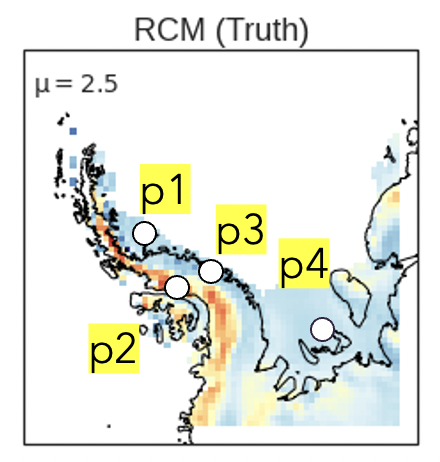
\includegraphics[width=\textwidth]{doc/Thesis-latex/images/results/points_location.png}
            \caption[]%
            {{\small}}    
          \label{fig:points-location}
        \end{subfigure}
        \hfill
        \begin{subfigure}[b]{\columnwidth}  
            \centering 
           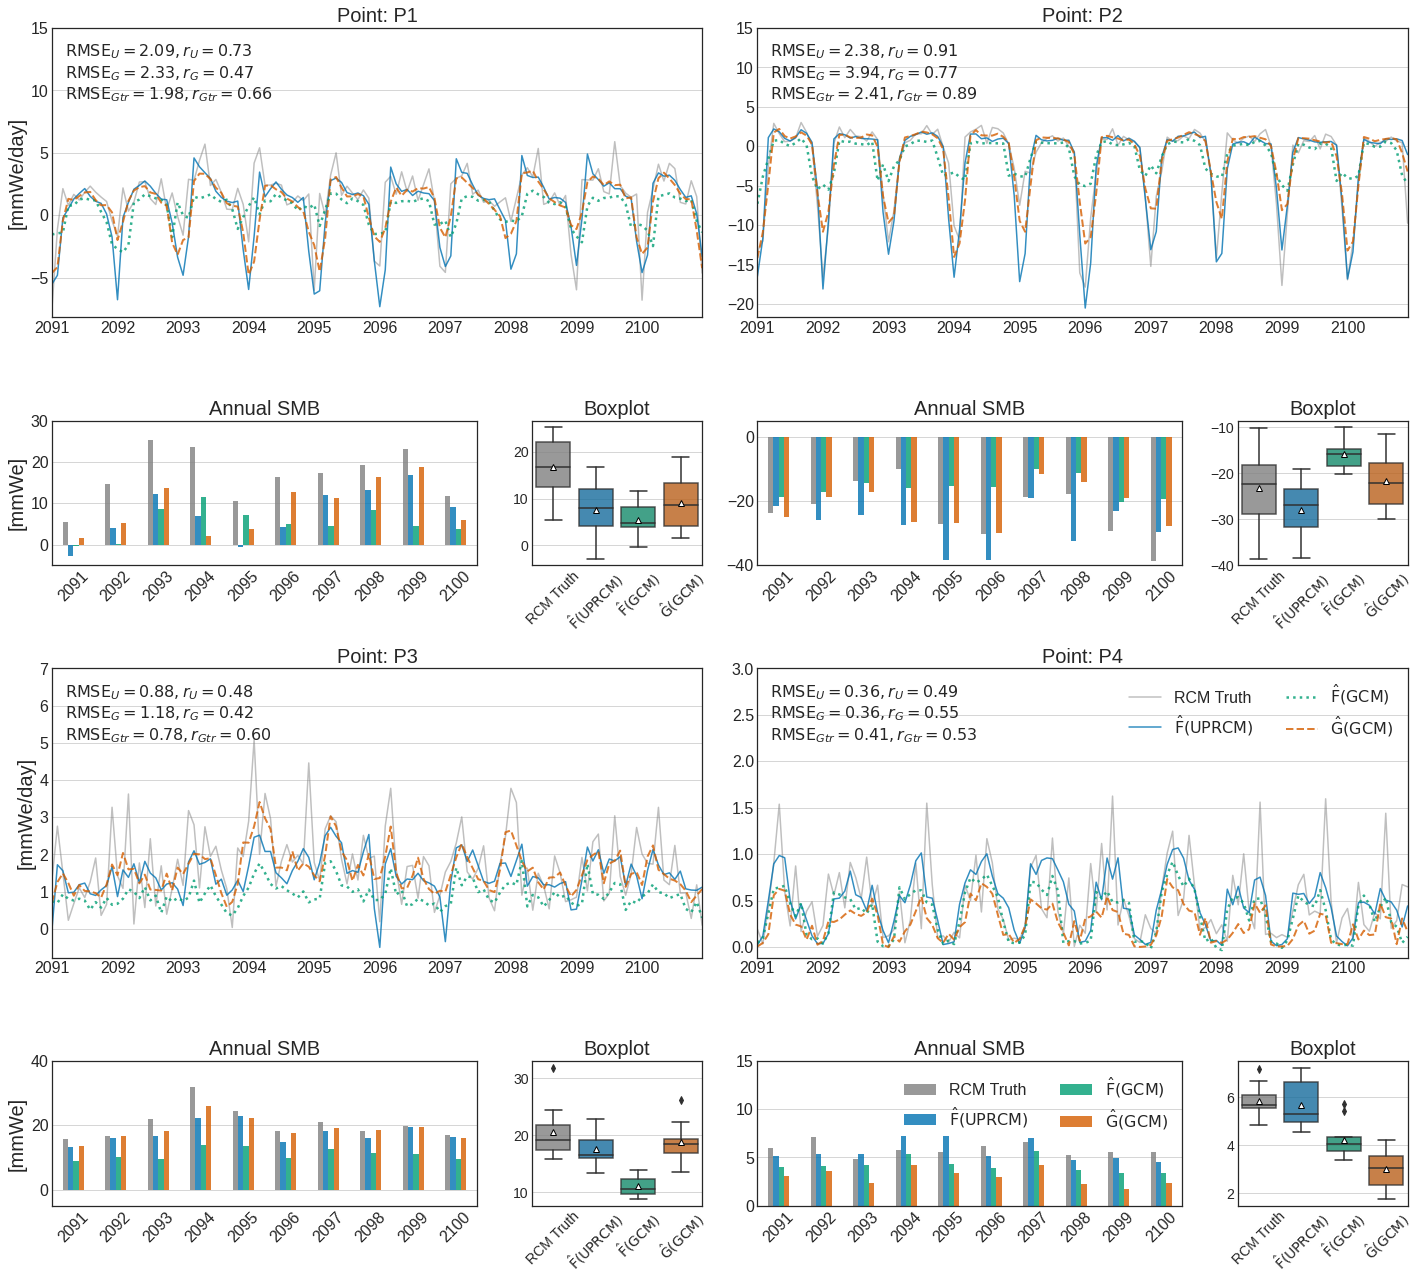
\includegraphics[width=\textwidth]{doc/Thesis-latex/images/results/timeseries_RCM_GCM.png}
            \caption[]%
            {{\small }}  
          \label{fig:timeseries-GCM-UPRCM}
        \end{subfigure}
        \hfill
        \caption[]
        {\small Predictions of Emulator trained on UPRCM ($\hat{F}$) or on GCM ($\hat{G}$) and using respectively UPRCM ($\operatorname{\hat{F}(UPRCM)}$) and GCM as low-resolution input ($\operatorname{\hat{F}(GCM)}$, $\operatorname{\hat{G}(GCM)}$). (b) Time-series of predictions of Emulator for four different geographical points (a) in target domain ($\mathcal{E})$). True SMB (grey), $\operatorname{\hat{F}(UPRCM)}$ (blue), $\operatorname{\hat{F}(GCM)}$ (green) and $\operatorname{\hat{G}(GCM)}$ (orange). Legend: temporal correlation ($\operatorname{r}$) and temporal RMSE ($\operatorname{RMSE}$) between the time-series of emulated and true SMB.. Test time-frame: 2090-2100. } 
        \label{fig:points-timeseries-GCM-UPRCM}
    \end{figure}

\subsection{Annual SMB predictions}

\begin{itemize}
    \item We also looked at the annual SMB predictions for both inputs. 
    \item Again we can see here that the model with GCM tends to underestimate the truth, while the RCM emulator comes closer to the truth in average
    \item Ref Fig.~\ref{fig:annual-SMB}
\end{itemize}





\subsection{Feature importance}

\subsection{Correlation}
\begin{figure}[tbp]
        \centering
        \begin{subfigure}[b]{\columnwidth}
            \centering 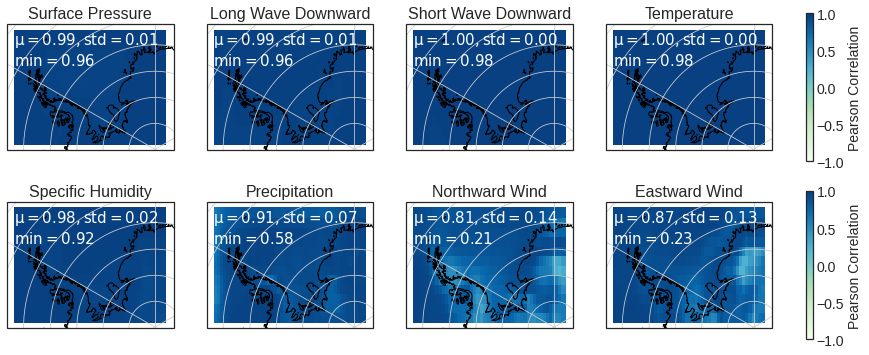
\includegraphics[width=\textwidth]{doc/Thesis-latex/images/results/temporalCorr_RCM_GCM.png}
            \caption[]%
            {{\small Temporal correlation over test period}}    
          \label{fig:temp-corr-GCM-UPRCM}
        \end{subfigure}
        \hfill
            \begin{subfigure}[b]{\columnwidth}
            \centering 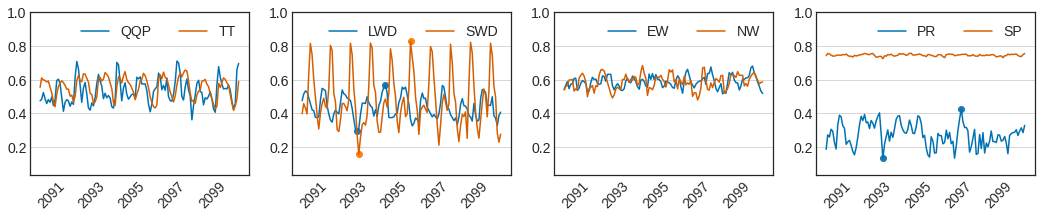
\includegraphics[width=\textwidth]{doc/Thesis-latex/images/results/spatialCorr_TS_RCM_GCM.png}
            \caption[]%
            {{\small Spatial correlation over test period}}    
          \label{fig:spatial-corr-GCM-UPRCM}
        \end{subfigure}
        \hfill
        \begin{subfigure}[b]{\columnwidth}  
            \centering 
            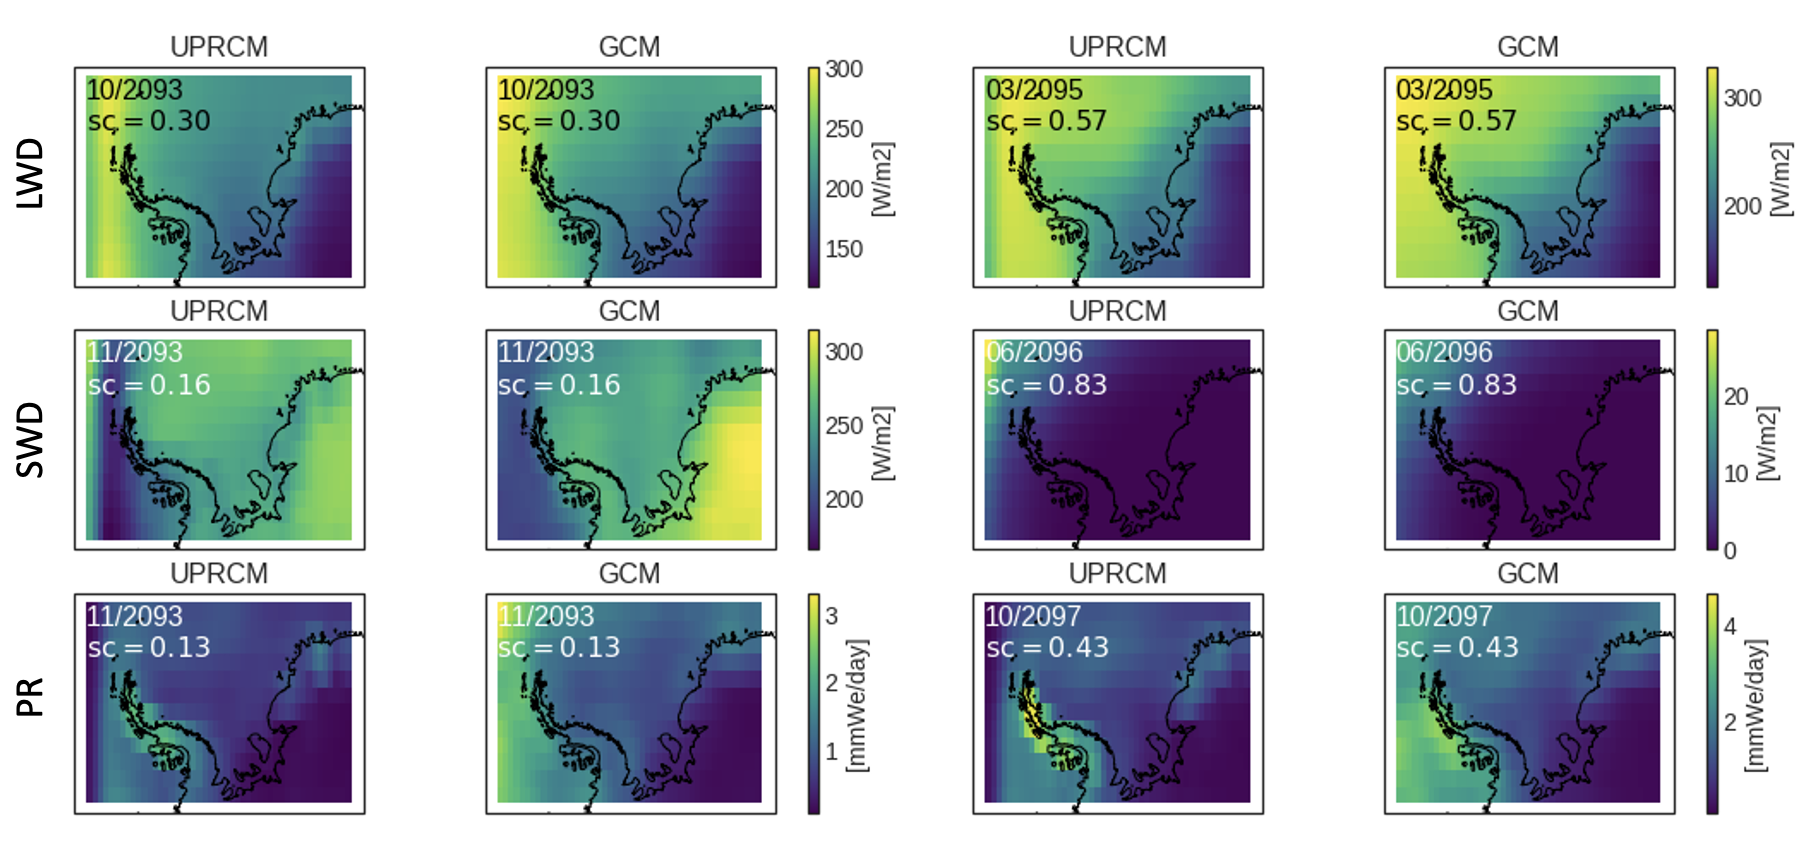
\includegraphics[width=\textwidth]{doc/Thesis-latex/images/results/spatialCorr_RCM_GCM.png}
            \caption[]%
            {{\small Spatial correlation for individual variables and months}}  \label{fig:spatial-corr-GCM-RCM-ex}
        \end{subfigure}
        \hfill
        \caption[]
        {\small Temporal (a) and spatial (b, c) correlation between UPRCM and GCM variables given as input to Emulator ($\hat{F}$) over target domain ($\mathcal{E})$) and test period (2090-2100). (a) Temporal correlation between UPRCM and GCM time-series for each point $p$ in target domain $\mathcal{E}$. Legend: mean ($\mu$) and standard deviation ($\operatorname{std}$) over $\mathcal{E}$. (b) Spatial correlation between UPRCM and GCM variables over $\mathcal{E}$ for each time step. (c) Example of time steps with lowest (left) and highest (right) spatial correlation ($\operatorname{sc}$) between UPRCM and GCM. Variables from top to bottom: long-wave downward radiation (LWD), short-wave downward radiation (SWD) and precipitation (PR).} 
        \label{fig:corr-GCM-RCM}
    \end{figure}


%%%%%%%%%%%%%%%%%%%%
\chapter{Discussion}
%%%%%%%%%%%%%%%%%%%%

In the evaluation you convince the reader that your design works as intended.
Describe the evaluation setup, the designed experiments, and how the
experiments showcase the individual points you want to prove.

This section is usually 5-10 pages.

\begin{itemize}
    \item Model from Doury is made for super resolution with LR as input. In our case don't have LR SMB available
    \item Temporal and spatial dis-correlation between GCM and RCM. Ref: Figure~\ref{fig:corr-GCM-RCM}
    \item Model doing its job but confused by different input when given GCM while trained on UPRCM
    \item Training on GCM directly ?
\end{itemize}



%%%%%%%%%%%%%%%%%%%%
\chapter{Conclusion}
%%%%%%%%%%%%%%%%%%%%

In the conclusion you repeat the main result and finalize the discussion of
your project. Mention the core results and why as well as how your system
advances the status quo.

\cleardoublepage
\phantomsection
\addcontentsline{toc}{chapter}{Bibliography}
\printbibliography

% Appendices are optional
\appendix
% %%%%%%%%%%%%%%%%%%%%%%%%%%%%%%%%%%%%%%
\chapter{Data processing}
\begin{figure}[!t]
  \centering
  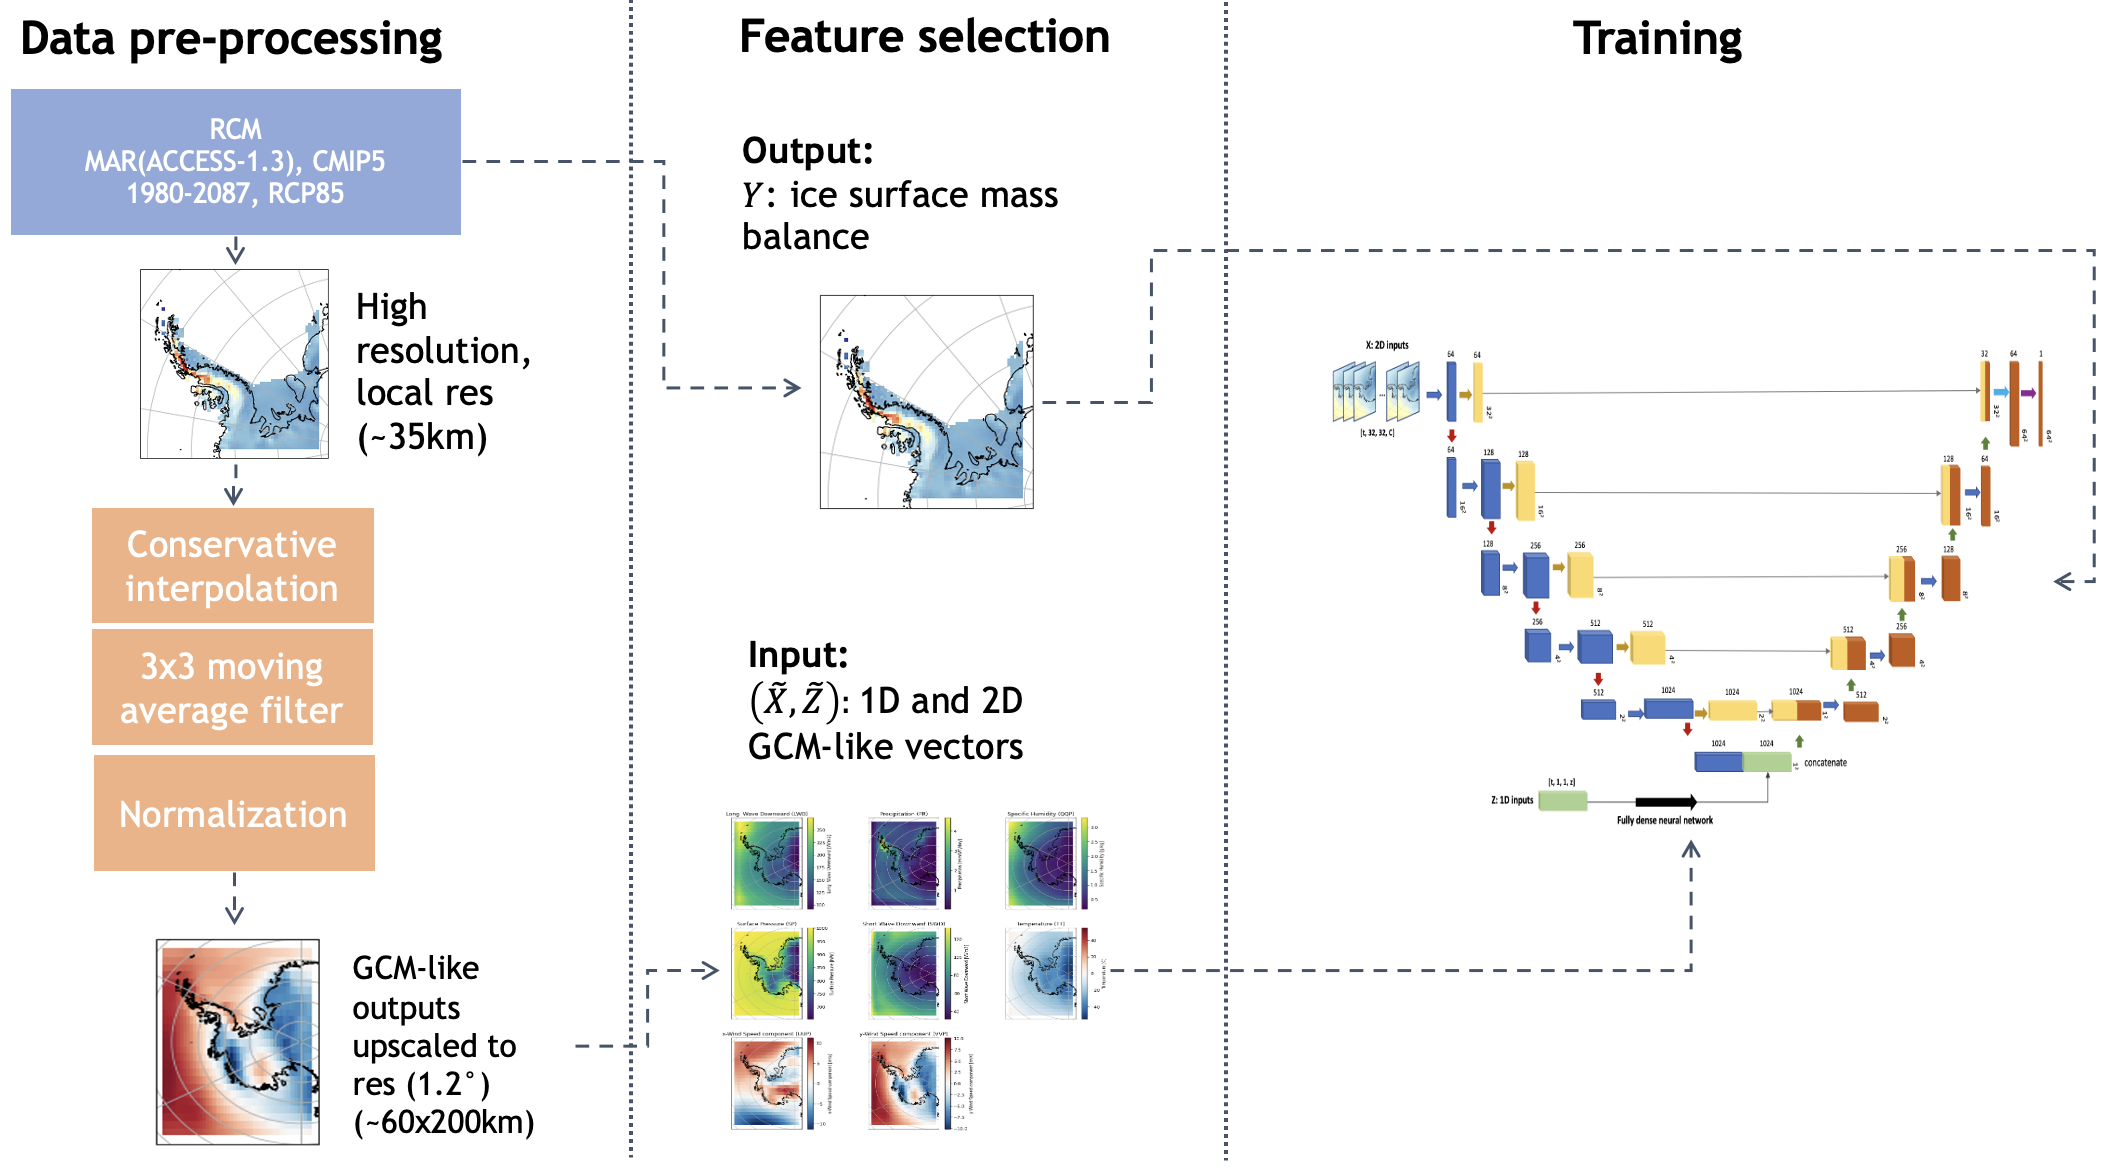
\includegraphics[width=\columnwidth]{images/data-flow.png}
  \caption []{\small Training data flow}
  \vspace{-3mm}
  \label{fig:training-data-flow}
\end{figure}
\section{Pre-processing of RCM}
\begin{itemize}
    \item  Because GCM data we have is monthly frequency, do monthly mean aggregation for RCM data.

\end{itemize}
\section{Pre-processing of GCM}
\chapter{Feature selection}
\section{Feature selection RCM}
\section{Feature selection GCM}

\chapter{Hyperparameter tuning}
% %%%%%%%%%%%%%%%%%%%%%%%%%%%%%%%%%%%%%%

\begin{table}[tbp]
    \centering
    \caption{}
    \renewcommand\arraystretch{1.5}
    \begin{tabular}{l>{\centering}p{0.1\linewidth}>{\centering}p{0.1\linewidth}>{\centering}p{0.05\linewidth}>{\centering}p{0.05\linewidth}>{\centering}p{0.05\linewidth}>{\centering}p{0.1\linewidth}>{\centering}p{0.05\linewidth}>{\raggedright\arraybackslash}p{0.05\linewidth}}
    \toprule
        Model & x & y & Batch size & Num epochs & Weight decay & learning rate & Train loss & Val loss \\ \toprule
        Simul 2 & (3, 500, 500) & (3, 500, 500) & 4 & 10 & 1e-3 & 0.01 & 0.5513 & 0.5490 \\ 
        Sim 3 & (3, 250, 250) & (3, 250, 250) & 20 & 10 & 1e-3 & 0.01 & 0.6505 & 0.6240 \\ 
        Sim 4 & (3, 250, 334) & (3, 250, 334) & 15 & 10 & 1e-3 & 0.01 & 0.6056 & 0.5875 \\ 
        Sim 5 & (3, 250, 334) & (3, 250, 334) & 15 & 10 & 1e-3 & 0.01 & 0.6043 & 0.5753 \\ 
        Sim 6 & (3, 250, 334) & (3, 250, 334) & 15 & 10 & 1e-3 & 0.01 & 0.4498 & 0.5015 \\ 
        Sim  7 & (3, 250, 334) & (3, 250, 334) & 15 & 10 & 1e-3 & 0.01 & 0.3511 & 0.3460 \\ 
        Sim  8  & (3, 250, 334) & (3, 250, 334) & 15 & 10 & 1e-3 & 0.01 & 0.6199 & 0.6041 \\ 
        Sim 9 & (3, 250, 334) & (3, 250, 334) & 15 & 10 & 1e-3 & 0.01 & 0.5916 & 0.5254 \\ \bottomrule
    \end{tabular}
        \subcaption*{\small Table~\ref{tab:phase1a}. Phase 1a. \textbf{Validation and training loss}: value at the end of the last epoch. \textbf{x and y}: input and output given to the model during training. }
            \label{tab:phase1a}
\end{table}
% In case you ever need an (optional) appendix.
%
% You need the following items:
% \begin{itemize}
% \item A box
% \item Crayons
% \item A self-aware 5-year old
% \end{itemize}

\end{document}